Chapter*{Modelos de Amplificadores Não Lineares} \label{apendix II}

\par Amplificadores de potência (PA) são dispositivos essenciais nas comunicações RF. Geralmente, apresentam um comportamento linear somente para um intervalo limitado de entrada: quanto maior for a amplitude deste sinal, mais próximo da saturação estará o PA, o que pode levar a distorção do sinal amplificado e limitar a eficiência energética. 
\par Fica claro que, ao projetar um sistema com amplificação, existirá uma troca entre linearidade e eficiência \cite{Bhat}. Para ilustrar essas afirmações, dois modelos de amplificadores são apresentados: um que desconsidera os efeitos de memória e outro que os leva em conta. 
 
\begin{enumerate} 
\item {Amplificadores Sem Memória} 

Amplificadores sem memória são dispositivos não lineares para os quais a saída não depende das amostras anteriores da entrada. Isso é o caso, geralmente, de amplificadores de estado sólido (SSA), os quais seguem o modelo Rapp \cite{Rapp}. Matematicamente, são representados por: 

\begin{equation} \label{x}
x(t) = A(t)e^{j\Psi(t)}
\end{equation}

em que $x$(t) é o sinal de entrada do amplificador de potência, com amplitude $A(t)$ e fase $\Psi(t)$. 

\par A saída vai ser dada como se segue \cite{Uilian2}:
\begin{equation} \label{y}
y(t) = G[A(t)] e^{\{j\Psi(t)+ \Phi[A(t)]\}} 
\end{equation}
na qual $G[A(t)]$ é o fator de conversão AM$/$AM e $\Phi[A(t)]$ o fator AM$/$PM do PA. Para o modelo Rapp, o comportamento da fase, contabilizado por \textit{$\Psi$(t)}, pode ser descartado \cite{Uilian2}. A parte importante é $G[A(t)]$: 

\begin{equation} 
\label{GA}
G(A)= \frac{\nu A}{\left[1+ \left(\frac{A}{A_0} \right)^{2p} \right]^{1/2p}} 
\end{equation}
em que $\nu$ é o ganho de pequenos sinais, $A_0$ é a amplitude de saturação e $p$ é o fator de \textit{smoothness} ("suavização"). 

Para os resultados encontrados nos capítulos 4 a 5, considerou-se $A_0 =1$ and $p=3$. A função de transferência (\ref{GA}) para estes parâmetros é exibida na Figura \ref{FTrans}: 

\begin{figure}[h!]
\centering
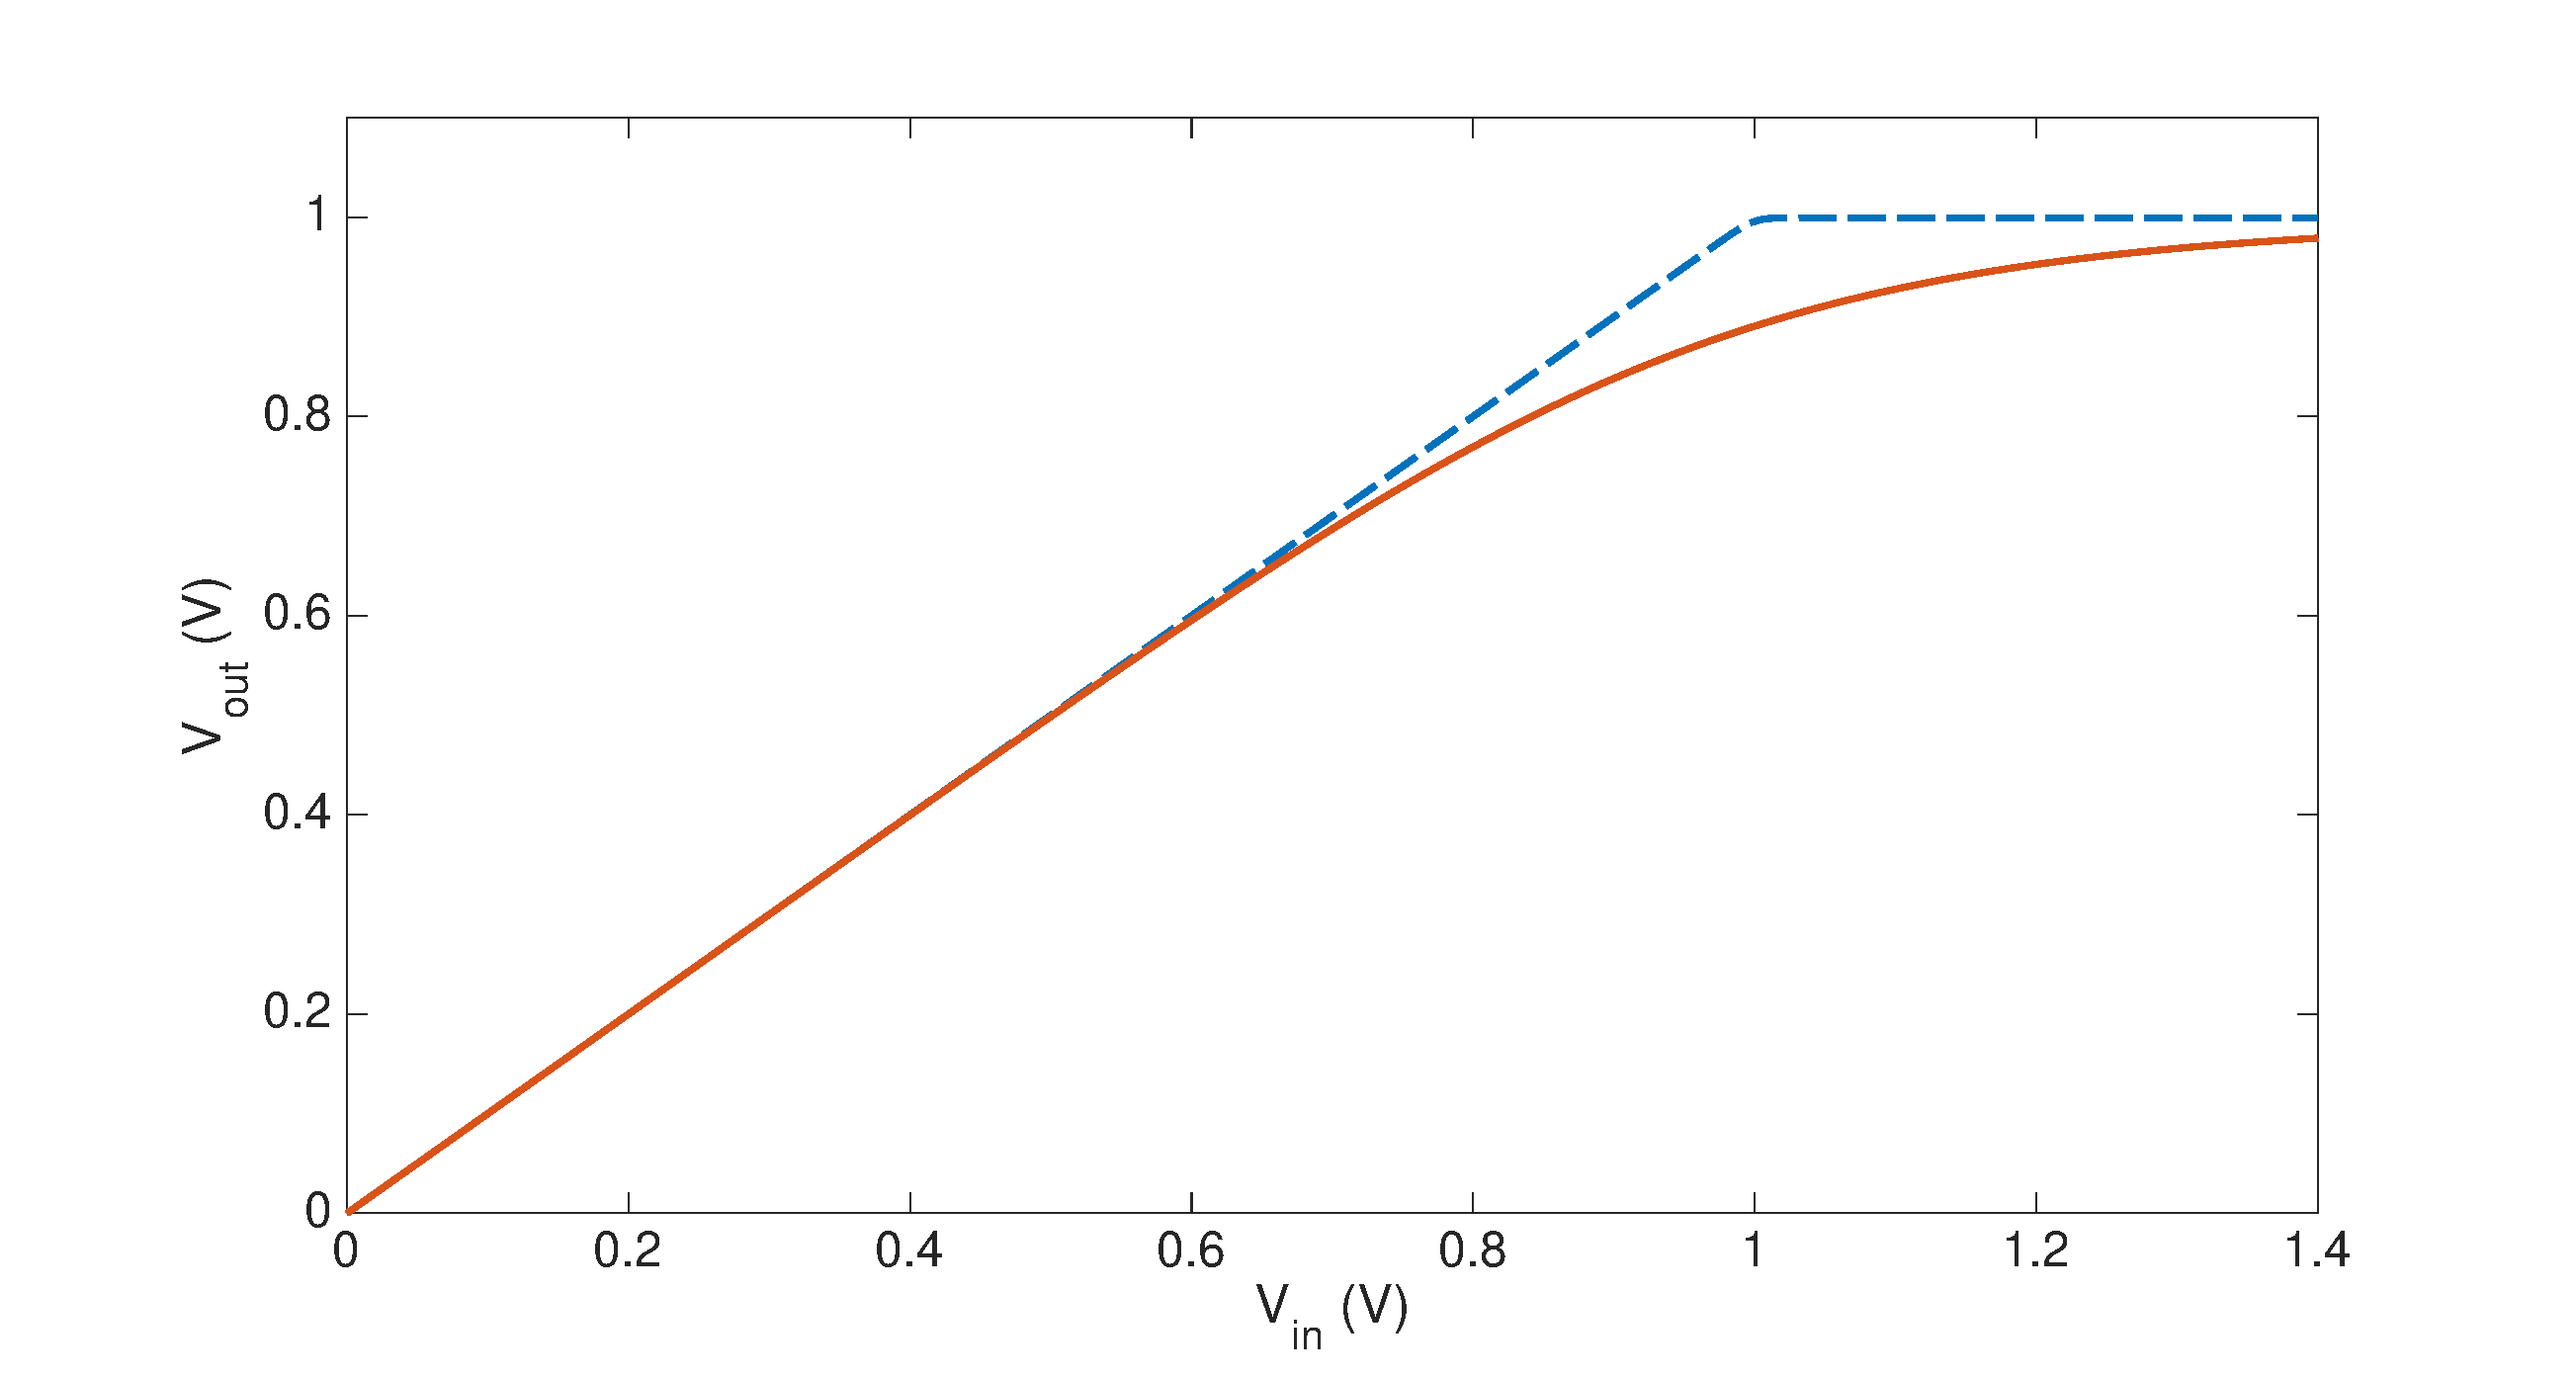
\includegraphics[width=3.5in]{HPA}
\caption{Transfer function of the non-linear amplifier.}
\label{FTrans}
\end{figure}

\item{Ampificadores de Potência com Memória} 
Nessa seção, efeitos de memória, que são comuns em amplificadores TWT são estudados. Para modela-los, será utilizada uma ferramenta matemática chamada Série de Volterra. Ems ua forma geral, esta é representada por: \cite{Morgan2006}: 

\begin{equation} 
\label{poly}
y(n)= \sum_{k=1}^{M-1}y_{k}(n),   
\end{equation}

em que 

\begin{equation} 
\label{kernel}
y_{k}(n)= \sum_{m_{1}=0}^{M-1}\dots\sum_{m_{k}=0}^{M-1}h_{k}(m_{1},\dots,m_{k})\prod_{l=1}^{k}y_{k}(n)  
\end{equation}

A equação (\ref{kernel}) é uma convolução multi-dimensional. O índice no tempo $m_{k}$ representa qual amostra do passado impacta no sinal do presente e $M$ é o comprimento da memória. Por simplicidade, no presente trabalho não se utilizou a série completa. Em \cite{Ding2004}, foi visto que é possível reduzir a equação do PA utilizando somente o polinômio de ordem ímpar: 

\begin{equation} 
\label{oddpoly}
y(n)= \sum_{k_{1}=0}^{K}\sum_{q=0}^{Q}c_{kq}z(n-q)|z(n-q)|^{k-1}
\end{equation}

Os coeficientes propostos foram extraídos, também de  \cite{Ding2004} e modelam um amplificador classe AB. Na análise, o comprimento de memória ($M$) é considerado $2$ e o grau do polinômio ($Q$) é $5$.  

\end{enumerate}